\todo{Write exciting new results in FTS along with questions left to verify.}
\section{Introduction}
Using a control contact draped over \ac{hBN} we demonstrated strong evidence for a normal mode on that exists purely on the hinge or side of the \ac{FTS} crystal\cite{Gray2019}. Recent works have called into question the exact topological nature of \ac{FTS} claiming the crystal is not a topological insulator but rather a topological semi-metal with buried Dirac nodes. In light of this it is crucial to obtain evidence with more experimental techniques to better understand the nature of the topology in the \ac{FTS} system. Indeed, the underlying physics which predicts the helical hinge mode also predicts the same mode to manifest as a bias-independent conductance plateau in a differential conductance measurement rather than the previously observed zero-bias conductance peak. To accomplish this, we investigate the effect edge quality has on the topological characteristics of \ac{FTS} as it has been previously shown that the quality of the crystal edge can have a drastic effect on its transport characteristics \todo{cite Andrea's work on different transport characteristics of graphene}. We find that when tunneling measurements are performed across pristine, high-symmetry crystalline edges bias-independent conductance plateaus are observed for biases below the superconducting gap energy while ``rough" edges do not exhibit such plateaus. Furthermore, these plateaus are consistent with \acl{PAR}.

\section{Observation of Bias-Independent Conductance Plateau}
The tunneling conductance of a normal-metal/superconductor interface can be modeled using the \ac{BTK} method. An in-depth discussion, as well as pseudo code for performing these simulations, can be found in \ref{app:ARfit}], however we will take some of the main results of these simulations for discussions here. The \ac{BTK} method on a standard \ac{BCS} s-wave superconductor predicts a bias-independent conductance plateau only when the strength of the potential barrier between the normal-metal and superconductor is exactly zero. Even slight deviations from a zero-strength barrier result in significant dips around zero-bias thus observing \ac{PAR} is exceedingly rare and typically only occurs only in extremely clean materials \todo{cite klein paper}. Therefore when \ac{PAR} is observed in a system it is usually due to an underlying mechanism which causes the incoming carriers to ignore the barrier completely. With this in mind, \ac{PAR} has three unique identifiers in a differential conductance spectrum: a perfectly flat plateau, the plateau is at twice the conductance of the normal state, and the plateau extends out to the superconducting energy gap. 
\begin{figure}
    \centering
    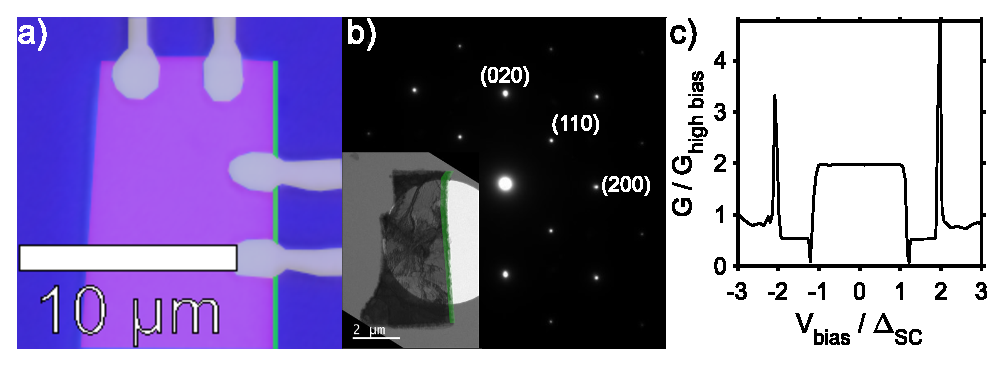
\includegraphics[width = \textwidth]{Chap4/Figures/DeviceFab.eps}
    \caption{a) False color optical image of a representative device with a straight (100) edge. b) \ac{TEM} diffraction pattern demonstrating the (100) edge. Inset shows the flake measured as well as the diffraction aperture. c) Base temperature differential conductance curve.}
    \label{fig:PARDeviceFab}
\end{figure}
\begin{figure}
    \centering
    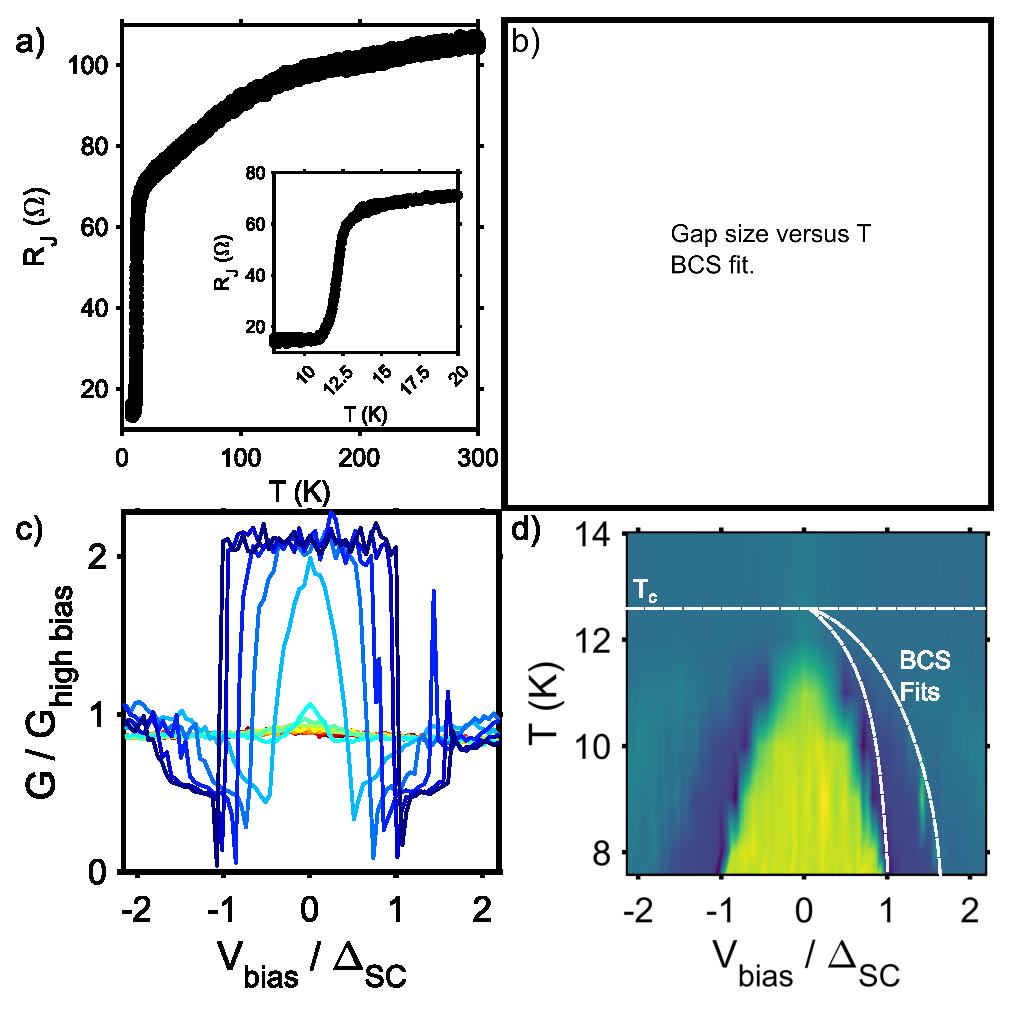
\includegraphics[width = \textwidth]{Chap4/Figures/Temperature.eps}
    \caption{Caption}
    \label{fig:PARTemp}
\end{figure}
\section{Magnetic Field Dependence}
\begin{figure}
    \centering
    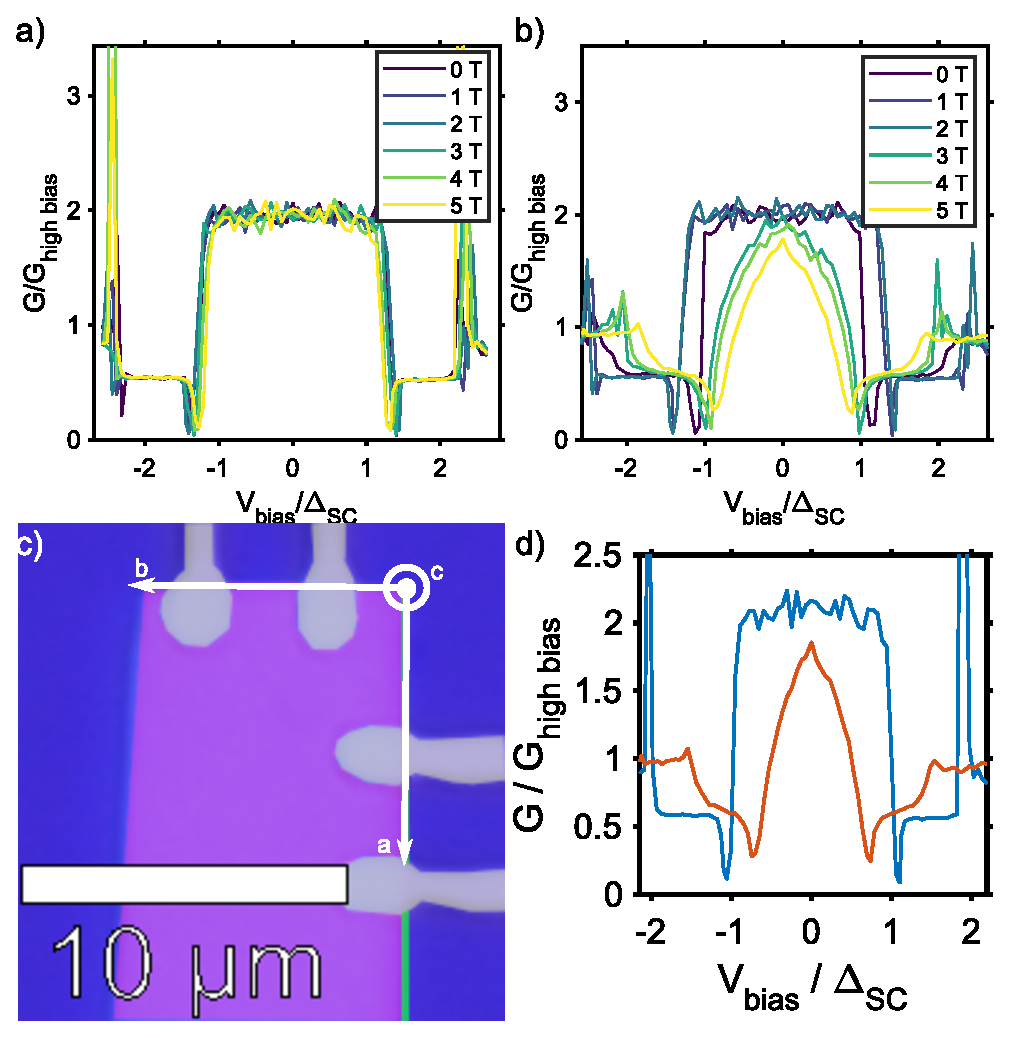
\includegraphics[width = \textwidth]{Chap4/Figures/MagneticField.eps}
    \caption{Caption}
    \label{fig:PARField}
\end{figure}
\section{Conclusion}